\documentclass[12pt]{article}
 
\usepackage[margin=1in]{geometry}
\usepackage{amsmath,amsthm,amssymb}
\usepackage{mathtools}
\DeclarePairedDelimiter{\ceil}{\lceil}{\rceil}
%\usepackage{mathptmx}
\usepackage{accents}
\usepackage{comment}
\usepackage{graphicx}
\usepackage{IEEEtrantools}
 \usepackage{float}
 
\newcommand{\N}{\mathbb{N}}
\newcommand{\Z}{\mathbb{Z}}
\newcommand{\R}{\mathbb{R}}
\newcommand{\Q}{\mathbb{Q}}
\newcommand*\conj[1]{\bar{#1}}
\newcommand*\mean[1]{\bar{#1}}
\newcommand\widebar[1]{\mathop{\overline{#1}}}


\newcommand{\cc}{{\mathbb C}}
\newcommand{\rr}{{\mathbb R}}
\newcommand{\qq}{{\mathbb Q}}
\newcommand{\nn}{\mathbb N}
\newcommand{\zz}{\mathbb Z}
\newcommand{\aaa}{{\mathcal A}}
\newcommand{\bbb}{{\mathcal B}}
\newcommand{\rrr}{{\mathcal R}}
\newcommand{\fff}{{\mathcal F}}
\newcommand{\ppp}{{\mathcal P}}
\newcommand{\eps}{\varepsilon}
\newcommand{\vv}{{\mathbf v}}
\newcommand{\ww}{{\mathbf w}}
\newcommand{\xx}{{\mathbf x}}
\newcommand{\ds}{\displaystyle}
\newcommand{\Om}{\Omega}
\newcommand{\dd}{\mathop{}\,\mathrm{d}}
\newcommand{\ud}{\, \mathrm{d}}
\newcommand{\seq}[1]{\left\{#1\right\}_{n=1}^\infty}
\newcommand{\isp}[1]{\quad\text{#1}\quad}
\newcommand*\diff{\mathop{}\!\mathrm{d}}

\DeclareMathOperator{\imag}{Im}
\DeclareMathOperator{\re}{Re}
\DeclareMathOperator{\diam}{diam}
\DeclareMathOperator{\Tr}{Tr}
\DeclareMathOperator{\cis}{cis}

\def\upint{\mathchoice%
    {\mkern13mu\overline{\vphantom{\intop}\mkern7mu}\mkern-20mu}%
    {\mkern7mu\overline{\vphantom{\intop}\mkern7mu}\mkern-14mu}%
    {\mkern7mu\overline{\vphantom{\intop}\mkern7mu}\mkern-14mu}%
    {\mkern7mu\overline{\vphantom{\intop}\mkern7mu}\mkern-14mu}%
  \int}
\def\lowint{\mkern3mu\underline{\vphantom{\intop}\mkern7mu}\mkern-10mu\int}




\newenvironment{theorem}[2][Theorem]{\begin{trivlist}
\item[\hskip \labelsep {\bfseries #1}\hskip \labelsep {\bfseries #2.}]}{\end{trivlist}}
\newenvironment{lemma}[2][Lemma]{\begin{trivlist}
\item[\hskip \labelsep {\bfseries #1}\hskip \labelsep {\bfseries #2.}]}{\end{trivlist}}
\newenvironment{exercise}[2][Exercise]{\begin{trivlist}
\item[\hskip \labelsep {\bfseries #1}\hskip \labelsep {\bfseries #2.}]}{\end{trivlist}}
\newenvironment{problem}[2][Problem]{\begin{trivlist}
\item[\hskip \labelsep {\bfseries #1}\hskip \labelsep {\bfseries #2.}]}{\end{trivlist}}
\newenvironment{question}[2][Question]{\begin{trivlist}
\item[\hskip \labelsep {\bfseries #1}\hskip \labelsep {\bfseries #2.}]}{\end{trivlist}}
\newenvironment{corollary}[2][Corollary]{\begin{trivlist}
\item[\hskip \labelsep {\bfseries #1}\hskip \labelsep {\bfseries #2.}]}{\end{trivlist}}

\newenvironment{solution}{\begin{proof}[Solution]}{\end{proof}}
 
\begin{document}
 
% --------------------------------------------------------------
%                         Start here
% --------------------------------------------------------------
\title{Math 120TC Homework 2}
\author{Ethan Martirosyan}
\date{\today}
\maketitle
\hbadness=99999
\hfuzz=50pt
\section*{Problem 1}
We prove this by induction on $m$. Let $m = 1$. Then we must show that $X_{1,2}$ is $0$ dimensional. This is intuitively clear since each simplex can only contain one vertex. Thus, we know that $X_{m,m+1}$ is $m-1$ dimensional when $m = 1$. Next, we may suppose that $X_{m,m+1}$ is $m-1$ dimensional for $m\geq 1$. We claim that $X_{m+1,m+2}$ is $m$ dimensional. We may delete one row and one column from $X_{m+1,m+2}$ to recover $X_{m,m+1}$. By the induction hypothesis, we know that this has dimension $m-1$. That is, any simplex in $X_{m,m+1}$ can have a maximum of $m$ vertices. When we add the one row and one column back, there is one more vertex that we can add to obtain $m+1$ vertices in that simplex. Thus $X_{m+1,m+2}$ is $m$ dimensional. By induction, we may conclude that $X_{m,m+1}$ is $m-1$ dimensional for all $m$.
\newpage
\section*{Problem 2}
We claim that $X_{m,m+1}$ has the property that if the boundary of an $m-1$ chain is $0$, then the $m-1$ chain is either $0$ or it consists of all $m-1$ simplices. We will prove the contrapositive. That is, we may suppose that the $m-1$ chain $A$ is not $0$ and that it does not contain all the $m-1$ simplices. We aim to show that $\partial{A} \neq 0$. By assumption, we know that there must be some $m-1$ simplex $B \in A$ and some $m-1$ simplex $C \not \in A$. Then, there must be some $m-1$ simplex $D \in A$ adjacent to $C$. Let us denote the $m-2$ facet bounded by $D$ and $C$ by $F$. We claim that $F \in \partial{A}$. To show this, it suffices to prove that $F$ is not a facet of any $m-1$ simplices besides $C$ and $D$. However, this fact follows easily from problem $1$, which states that $X_{m,m+1}$ is $m-1$ dimensional. Thus, we have $F \in \partial{A}$, so we know that $\partial{A} \neq 0$. This proves the problem. Let us draw this in the case of $X_{3,4}$:
\begin{figure}[H]
\centering
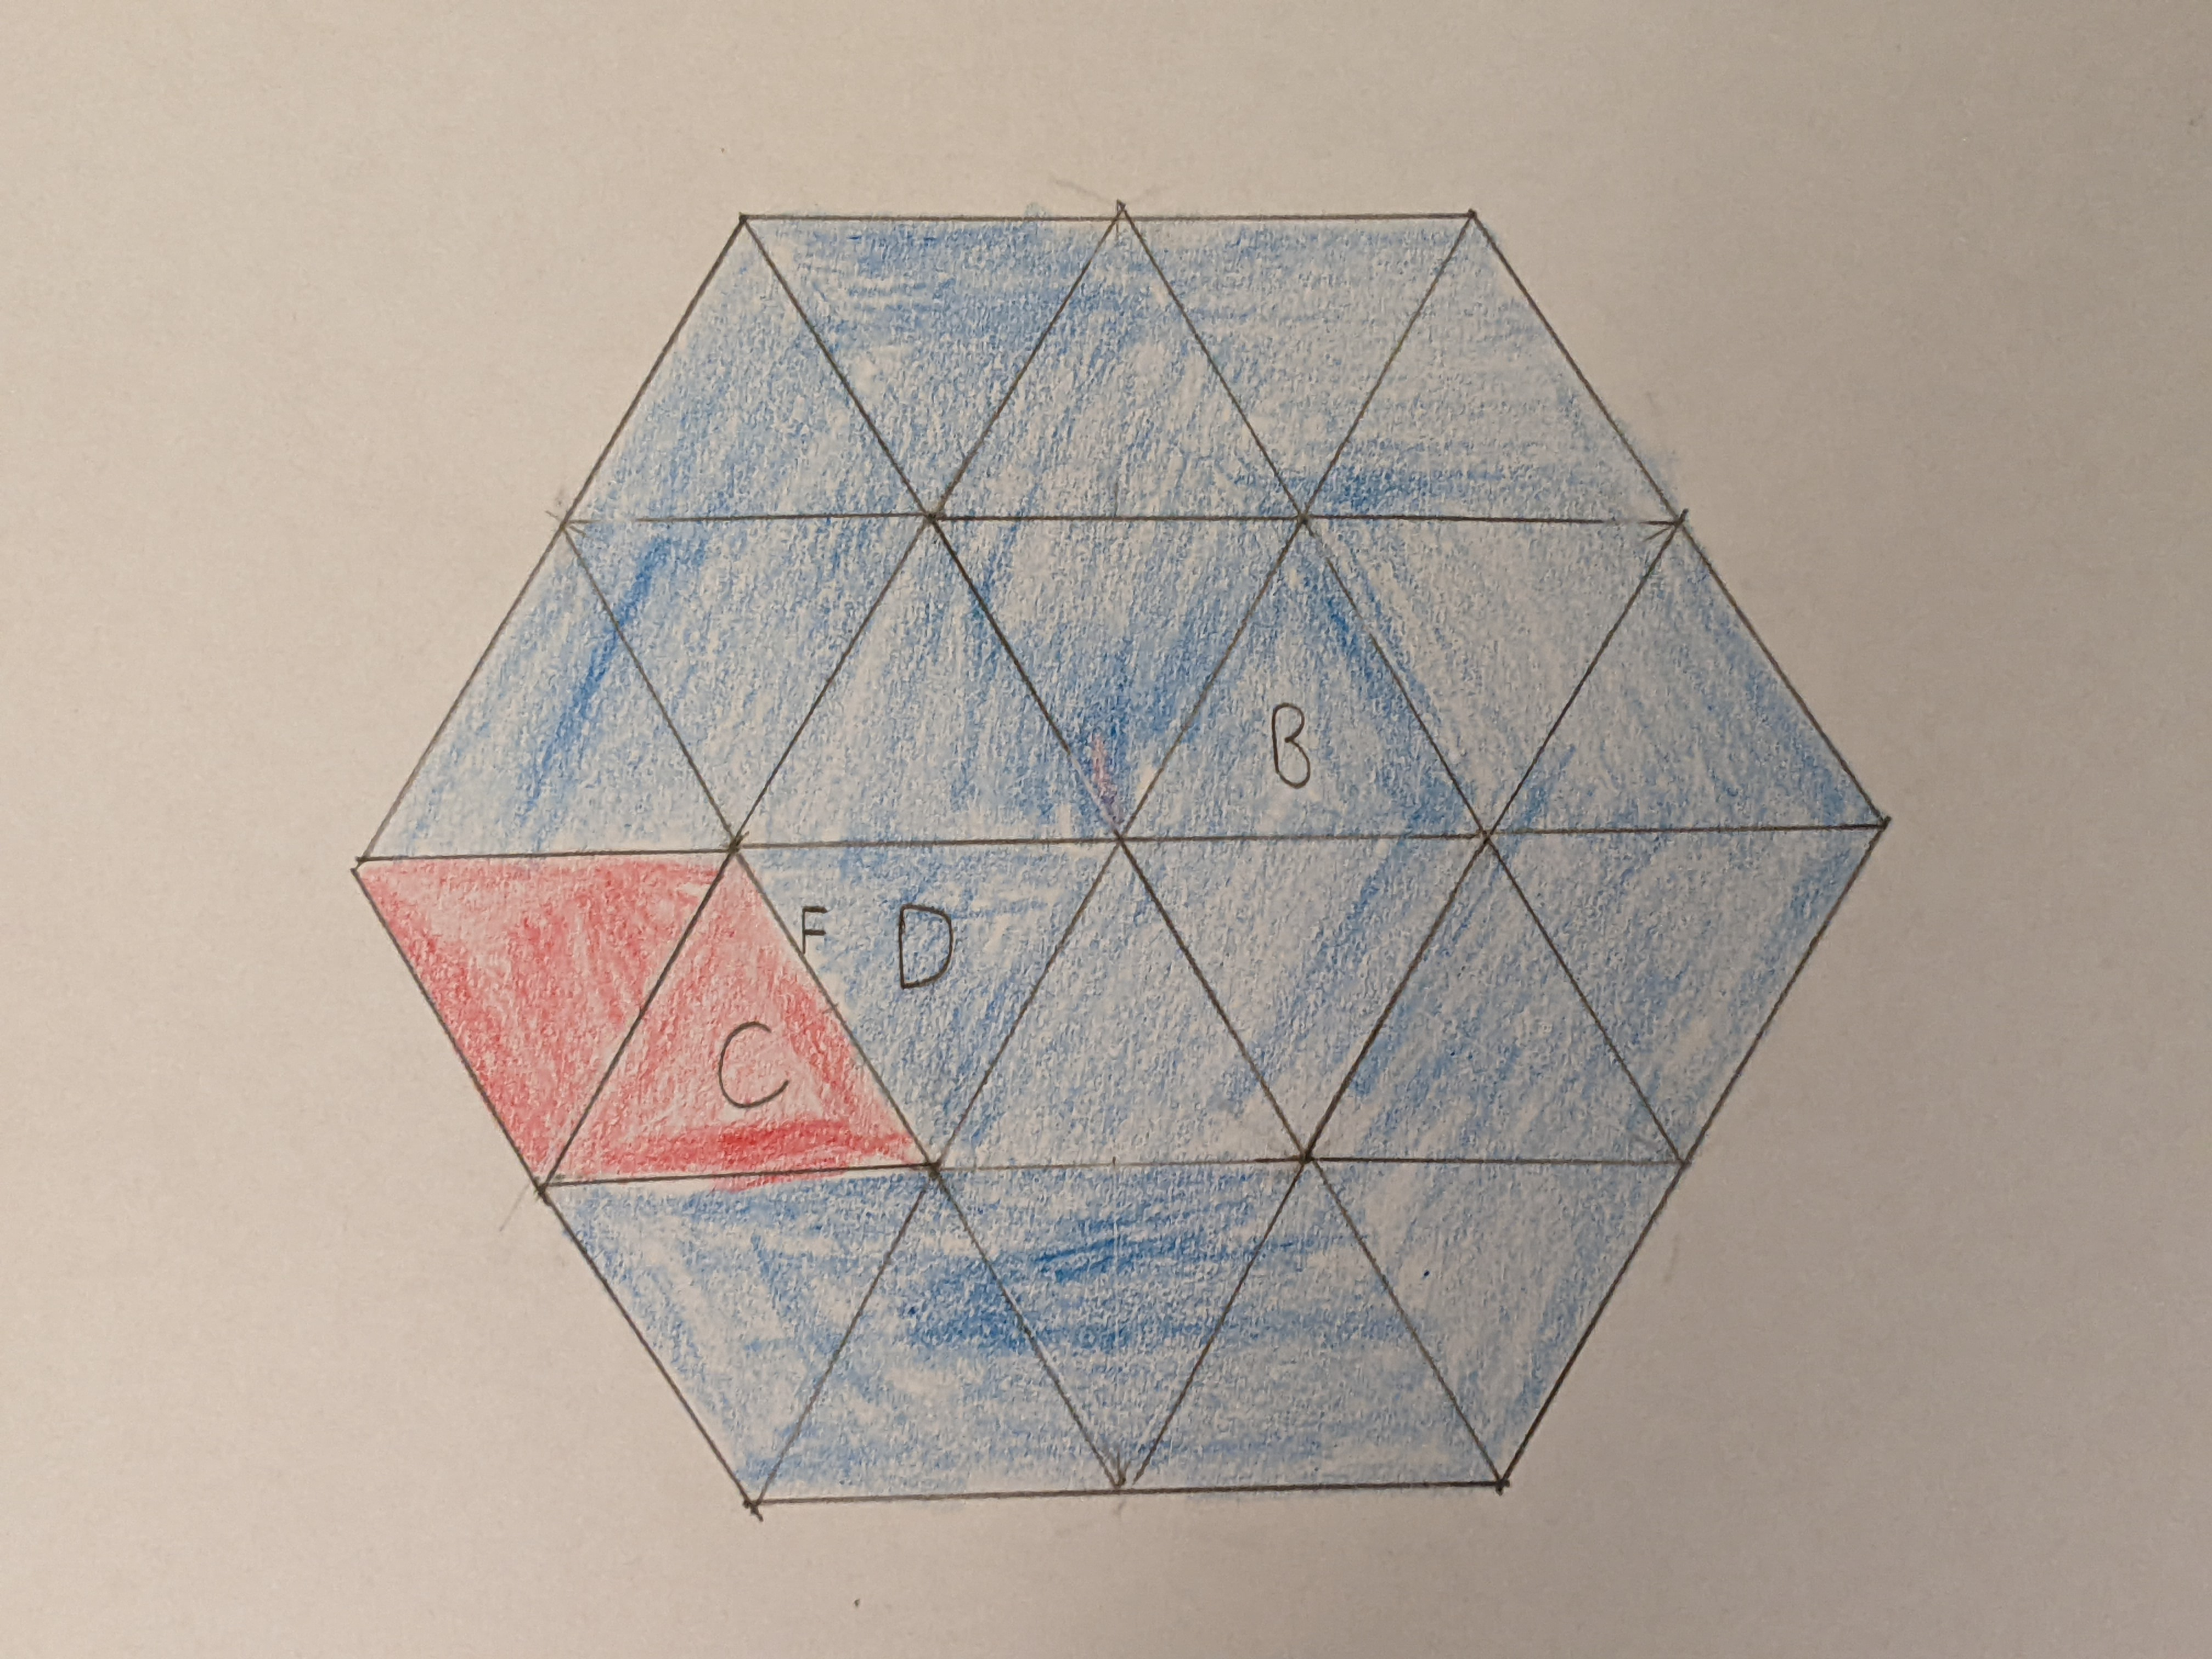
\includegraphics[width=\textwidth]{Image1}
\end{figure}
\noindent The blue simplices are in $A$, and the red simplices are not in $A$.
\newpage
\section*{Problem 3}
In any finite graph, the number of vertices of odd degree is even. This can be seen from the fact that the sum of all the degrees of all the vertices is twice the number of edges. Thus the sum of all the degrees of all the vertices is even. Let $S$ be the sum of all the degrees of all the vertices. Then, we may write $S = 2s$, where $s$ is the number of edges. Furthermore, it is obvious that the sum of all the degrees of all the vertices with even degree is even (let us denote this sum by $T$ so that $T = 2t$ for some integer $t$). Let $O$ denote the sum of all the degrees of all the vertices with odd degree. Then we have $O + T = S$ so that $O = 2(s-t)$. 
From this, we deduce that $O$ is even. We may conclude that the number of vertices of odd degree must be even (this is the only way for $O$ to be even). 

Now, we let $C$ denote an antipodally symmetric $1$ chain. We claim that $\partial{C}$ contains an even number of pairs of antipodal points. We may write $C = D + E$, where $D$ and $E$ are antipodal. If we view $D$ as a graph, then we know that it has an even number of vertices of odd degree. That is, $D$ contains an even number of points which are connected to an odd number of edges. By definition, $\partial{D}$ consists of an even number of points. Now, we claim that $\partial{C} = \partial{D} + \partial{E}$ contains an even number of pairs of antipodal points. If $\partial{D} \cap \partial{E} = \varnothing$, then we are already done. If their intersection is not $0$, then we note that it contains an even number of points. This is evident from the assumption that $C$ is antipodally symmetric. That is, if $\partial{D}$ intersects $\partial{E}$ in one point, then there must be another point of intersection that is antipodal to the first point of intersection. Furthermore, this antipodal pair counts for both $\partial{E}$ and $\partial{D}$. Thus we may conclude that $\partial{C}$ contains an even number of pairs of antipodal points.
\end{document} 